%======================================================================%
% Filename: Article.tex
% Project: Insight Journal Article - ManagedITK
% Author: Dan Mueller - d.mueller[at]qut.edu.au, dan.muel[at]gmail.com
%----------------------------------------------------------------------%
% Description:
% This artcile is for the Insight Journal.
% It describes the .NET CLR (ie. C#) wrappers for ITK.
%======================================================================%
\documentclass{InsightArticle}

%\usepackage{times}							%Font
%\usepackage{newcent}						%Font
%\usepackage{pslatex}						%Font
%\usepackage{lmodern}						%Font
%\usepackage{palatino}					%Font
%\usepackage{bookman}						%Font
\usepackage{amsfonts}						%Maths fonts
\usepackage{amssymb}						%Maths symbols
\usepackage{listing}						%Used for list of listings
\usepackage{listings}						%List program code source
%\usepackage{lstpatch}						%List program code source
\usepackage{subfigure}				  %For subfigures
\usepackage{graphicx}						%Graphics
\usepackage[dvipdfm=true,
			bookmarks=true, 
			bookmarksopen=true,
			bookmarksnumbered=true, 
			backref=section,
			colorlinks=true,
			linkcolor={blue},
			citecolor={blue},
			urlcolor={blue}]{hyperref}

%Set default font
%\renewcommand{\familydefault}{\rmdefault}	%Roman
\renewcommand{\familydefault}{\sfdefault}	%Sans serif
%\renewcommand{\familydefault}{\ttdefault}	%Typewriter

%Keywords
\newcommand{\keywords}[1]{\noindent\textbf{Keywords:}\it{\ #1}}

%Add images path
\graphicspath{{images/}}

%Code definitions
\def\code#1{\texttt{#1}}

%Create indent for description
\newenvironment{indentdescription}
               {\list{}{\leftmargin \leftmargin}%
                \item\relax}
               {\endlist}
               
%Allow symbol footnotes
\long\def\symbolfootnote[#1]#2{\begingroup%
\def\thefootnote{\fnsymbol{footnote}}\footnote[#1]{#2}\endgroup}                    

%Create conditional to include or exclude figures 
%(saves time during debug compilation).
\makeatletter
\newif\if@includefigs@
\@includefigs@true

%======================================================================%
%                   F r o n t   M a t t e r                            % 
%======================================================================%
% The title should be descriptive enough for people to be able to find
% the relevant document.
\title{ManagedITK: .NET Wrappers for ITK}

% Increment the release number whenever significant changes are made.
% The author and/or editor can define 'significant' however they like.
\release{3.6.0.2}

% Name and affiliation
\author{Dan Mueller$^{\scriptscriptstyle\textsf{1}}$}
\authoraddress{$^{\textsf{1}}$Philips Healthcare, PII Development, Best, Netherlands}

% Set custom header style
\pagestyle{fancy}								
\fancyhead{} 			% clear all header fields
\fancyhead[L]{\textsf{ManagedITK: .NET Wrappers for ITK}}
\fancyhead[R]{\textsf{\thepage}}
\fancyfoot{} 			% clear all footer fields

% Document
\begin{document}

%Set up listing environment
\definecolor{listcomment}{rgb}{0.0,0.5,0.0}
\definecolor{listkeyword}{rgb}{0.0,0.0,0.5}
\definecolor{listnumbers}{gray}{0.65}
\definecolor{listlightgray}{gray}{0.955}
\definecolor{listwhite}{gray}{1.0}


\newcommand{\lstset@csharp}
{
\lstset{frame = tb,
        framerule = 0.25pt,
        float,
        fontadjust,
        backgroundcolor={\color{listlightgray}},
        basicstyle = {\ttfamily\footnotesize},
        keywordstyle = {\ttfamily\color{listkeyword}\textbf},
        identifierstyle = {\ttfamily},
        commentstyle = {\ttfamily\color{listcomment}\textit},
        stringstyle = {\ttfamily},
        showstringspaces = false,
        showtabs = false,
        numbers = left,
        numbersep = 6pt,
        numberstyle={\ttfamily\color{listnumbers}},
        tabsize = 2,
        language=[Sharp]C,
        floatplacement=!h
        }
}

\newcommand{\lstset@csharpexample}
{
\lstset{frame = none,
        framerule = 0.0pt,
        float,
        fontadjust,
        backgroundcolor={\color{listlightgray}},
        basicstyle = {\ttfamily\footnotesize},
        keywordstyle = {\ttfamily\color{listkeyword}\textbf},
        identifierstyle = {\ttfamily},
        commentstyle = {\ttfamily\color{listcomment}\textit},
        stringstyle = {\ttfamily},
        showstringspaces = false,
        showtabs = false,
        numbers = left,
        numbersep = 6pt,
        numberstyle={\ttfamily\color{listnumbers}},
        tabsize = 2,
        language=[Sharp]C,
        floatplacement=!h
        }
}

\newcommand{\lstset@console}
{
\lstset{frame = none,
        framerule = 0pt,
        float,
        fontadjust,
        backgroundcolor={\color{listwhite}},
        basicstyle = {\ttfamily\footnotesize},
        keywordstyle = {\ttfamily},
        identifierstyle = {\ttfamily},
        commentstyle = {\ttfamily},
        stringstyle = {\ttfamily},
        showstringspaces = false,
        showtabs = false,
        numbers = none,        
        tabsize = 2,
        floatplacement=!h
        }
}

\newcommand{\lstset@python}
{
\lstset{frame = tb,
        framerule = 0.25pt,
        float,
        fontadjust,
        backgroundcolor={\color{listlightgray}},
        basicstyle = {\ttfamily\footnotesize},
        keywordstyle = {\ttfamily\color{listkeyword}\textbf},
        identifierstyle = {\ttfamily},
        commentstyle = {\ttfamily\color{listcomment}\textit},
        stringstyle = {\ttfamily},
        showstringspaces = false,
        showtabs = false,
        numbers = left,
        numbersep = 6pt,
        numberstyle={\ttfamily\color{listnumbers}},
        tabsize = 2,
        language=Python,
        floatplacement=!h
        }
}
\newcommand{\lstset@pythonexample}
{
\lstset{frame = none,
        framerule = 0pt,
        float,
        fontadjust,
        backgroundcolor={\color{listlightgray}},
        basicstyle = {\ttfamily\footnotesize},
        keywordstyle = {\ttfamily\color{listkeyword}\textbf},
        identifierstyle = {\ttfamily},
        commentstyle = {\ttfamily\color{listcomment}\textit},
        stringstyle = {\ttfamily},
        showstringspaces = false,
        showtabs = false,
        numbers = left,
        numbersep = 6pt,
        numberstyle={\ttfamily\color{listnumbers}},
        tabsize = 2,
        language=Python,
        floatplacement=!h
        }
}

\newcommand{\lstset@make}
{
\lstset{frame = tb,
        framerule = 0.25pt,
        float,
        fontadjust,
        backgroundcolor={\color{listlightgray}},
        basicstyle = {\ttfamily\footnotesize},
        keywordstyle = {\ttfamily\color{listkeyword}\textbf},
        identifierstyle = {\ttfamily},
        commentstyle = {\ttfamily\color{listcomment}\textit},
        stringstyle = {\ttfamily},
        showstringspaces = false,
        showtabs = false,
        numbers = left,
        numbersep = 6pt,
        numberstyle={\ttfamily\color{listnumbers}},
        tabsize = 2,
        language=make,
        floatplacement=!h
        }
}

% Show the title
\maketitle

% Make the title page header/footer empty
\thispagestyle{empty}

%======================================================================%
%                       A b s t r a c t                                % 
%======================================================================%
\begin{abstract}
\noindent
ManagedITK generates wrappers around ITK for .NET languages.
These wrappers can be used with any CLR language, 
including C\#, VB.NET, IronPython, and others.
ManagedITK is useful for a number of reasons,
including the ability to rapidly create graphical user interfaces
using Windows Forms (also known as \code{System.Windows.Forms}).
Full source code and many in-depth examples accompany this article.
Pre-compiled .NET assemblies can also be downloaded for easy
integration into standalone C\# applications.
\\
\\
\keywords{C\#, C++/CLI, .NET, CLR, ITK, medical image processing}

\end{abstract}

%======================================================================%
%                     M a i n   M a t t e r                            % 
%======================================================================%
%\tableofcontents

%----------------------------------------------------------------------%
% Section
%----------------------------------------------------------------------%
\section{Introduction}

The Insight Toolkit (ITK) \cite{Yoo2002a} is an open-source software system 
designed for image segmentation and registration --- particularly for medical images.
ITK is implemented in C++ and supports multiple platforms including
Windows, Unix, MacOSX, etc. The toolkit is organised in a data-flow architecture:
process objects (eg. filters) consume data objects (eg. images).
The toolkit is implemented using generic programming principles, whereby
objects are templated over different types at compile-time. 
%
The architecture and design of ITK, together with the complied C++ implementation,
provides for efficiency, speed, and flexibility.
However, interpretive or scripting languages are useful for rapidly prototyping 
applications and developing graphical user interfaces (GUIs).
ITK has recently upgraded it's wrapping system to WrapITK \cite{WrapITK}.

WrapITK produces automatically generated wrappers for common
ITK objects using CableSwig\footnote{Cable Automates Bindings for Language Extension 
(Cable) Simplified Wrapper and Interface Generator (Swig): %
\href{http://www.itk.org/HTML/CableSwig.html}{http://www.itk.org/HTML/CableSwig.html}}.
SWIG\footnote{Simplified Wrapper and Interface Generator: \href{http://www.swig.org/}{http://www.swig.org/}}, 
upon which CableSwig is built, supports the generation of wrappers from C++ to various
scripting languages including Perl, PHP, Python, Tcl, Ruby and PHP, as well as other
non-scripting languages such as C\#, Lisp, Java, Modula-3 and OCAML. 
However, CableSwig derives from an old version of SWIG and
at the time of writing only supports Python, Java, and Tcl.
%
It is desirable to generate ITK wrappers for CLR\footnote{The CLR (Common Language Runtime) is the 
Microsoft Windows implementation of the CLI (Common Language Infrastructure). Basically it is a Windows
implementation of a virtual machine able to run CIL (Common Intermediate Language) bytecode.
See \figurename~\ref{fig:OverviewOfCLI}.} languages, 
such as C\#, VB.NET and IronPython.
The .NET CLR is a popular platform which provides a large body of pre-coded solutions to
common programming problems, including a powerful GUI application 
programming interface (API) known as \code{System.Windows.Forms} or simply Windows Forms.

This article describes ManagedITK --- 
a project which generates ITK wrappers for .NET CLR languages.
It extends (probably more accurately mangles) WrapITK,
but is a separate system which does not use CableSWIG or SWIG.
The generated wrappers are created in a semi-automated fashion, 
tailored to produce a set of managed classes with 
well-defined methods, properties, and events.
As such, the generated wrappers are not 100\% pure 
(ie. in some cases the ITK API has been altered to better fit the 
Common Language Infrastructure (CLI) architecture, 
especially with the addition of properties). 
The next section describes the features of ManagedITK,
providing a discussion of both advantages and disadvantages.
Following this, the use of the pre-compiled assemblies is discussed,
as well as the compilation process from the included source files.
The bulk of the remaining text is devoted to in-depth examples
demonstrating the nuts-and-bolts of using the .NET CLR wrappers.

%----------------------------------------------------------------------%
% Section
%----------------------------------------------------------------------%
\section{Features}

As with any engineering solution,
ManagedITK offers a number of benefits at the cost of various trade-offs.
The advantages of ManagedITK include:
\begin{description}
	\item[Rapid GUI Development:] 
	The Windows Forms library can be used to quickly
	and easily create graphical user interfaces which interact with ITK data
	and process objects.
	For examples see 
	Section~\ref{sec:Examples:Bitmap1},
	and
	Section~\ref{sec:Examples:BinaryThreshold1}.
	
	\item[Run-time Type Specification:] 
	Most ManagedITK objects provide ``runtime-type wrapper'' objects which
	can be used to specify the explicit type at run-time,
	rather than compile-time (as with the native C++ templates).
	For example, the \code{itkImage} class provides a runtime-type
	wrapper around the explicit types \code{itkImage\_UC2}, \code{itkImage\_SS2},
	\code{itkImage\_F2}, etc, allowing the user to choose the type
	at run-time.	
	
	\item[Simplified Event Handling:] 
	Native ITK events can be easily observed using managed \code{delegates}.
	See Section~\ref{sec:Examples:Sigmoid1} for more details.
	
	\item[Multi-language Support:] Supported languages include 
	C\#, 
	C++/CLI, 
	VB.NET, 
	IronPython\footnote{\href{http://www.codeplex.com/IronPython/Wiki/View.aspx}
							 {http://www.codeplex.com/IronPython/Wiki/View.aspx}}, 
	F\#\footnote{\href{http://research.microsoft.com/fsharp}
					  {http://research.microsoft.com/fsharp}}, 
	Chrome (Object Pascal)\footnote{\href{http://www.chromesville.com}
										 {http://www.chromesville.com}},
	and other languages which target the .NET CLR.
	
	\item[Object Browser and Auto-complete:] 
	The documentation from ManagedITK assemblies can be viewed in the 
	Object Browser to discover managed classes, methods, properties, and events.
	The Visual Studio auto-complete feature can be used to read documentation
	while coding. See \figurename~\ref{fig:FeatureObjectBrowser} and
	\figurename~\ref{fig:FeatureAutoComplete}.
\end{description}

Unfortunately ManagedITK suffers from a number of disadvantages:
\begin{description}
	\item[Windows Platform Only:] 
	ManagedITK has a dependency on the \code{vcredist} assemblies.
	These libraries are only supported by the Windows.NET CLR.
	
	\item[Memory Management:]
	The CLR is an interpreted architecture which uses a garbage collector (GC)
	to manage memory.
	As such, there are no guarantees regarding object finalization:
	the garbage collector reclaims memory as it sees fit.
	This means that even though an image may no longer be in scope,
	there is no guarantee that the native \code{itk::Image} resources have been
	freed.
	To help alleviate the issue, every ManagedITK object implements the
	\code{IDisposable} interface, providing a \code{Dispose()} 
	method\footnote{See 
	\href{http://msdn2.microsoft.com/en-us/library/aa730837(VS.80).aspx\#cplusclibp\_topic3}
	     {http://msdn2.microsoft.com/en-us/library/aa730837(VS.80).aspx\#cplusclibp\_topic3} for
	     more details.}.
	Calling this method forces the native object to free its resources,
	however --- in some respects --- this practice defeats the purpose of
	the \code{itk::SmartPointer}.
	In our experience it is not \emph{imperative} to call \code{Dispose()},
	nonetheless it has been provided to support deterministic finalization.
	
	\item[Virtual Memory Allocation:]
	Unfortunately we have found the use of virtual memory is limited
	in comparison to a native C++ implementation.
	In our experience, a process running on a system with 1 GB physical RAM can
	only allocate approximately 1 GB of memory.
	A process running on a system with 2+ GB physical RAM can allocate the full
	theoretical 2 GB of memory before an \code{OutOfMemoryException} is thrown.
	
	\item[Performance:]
	Most ManagedITK classes achieve similar performance to their native
	counterparts.
	However, a single managed-to-native transition (when managed code calls native code)
	reduces the execution speed.
	Optimal performance is achieved when such transitions are
	minimised\footnote{See
	\href{http://msdn2.microsoft.com/en-us/library/aa730837(VS.80).aspx\#cplusclibp\_topic5}
		 {http://msdn2.microsoft.com/en-us/library/aa730837(VS.80).aspx\#cplusclibp\_topic5} for
	more details.}.
	For most \code{itk::ProcessObjects} the \code{Update()} method encapsulates the
	processing, which inherently minimises these transitions.
	This means, for example, that a majority of managed \code{itk::ImageToImageFilter}
	subclasses will execute with similar speed to a natively compiled executable.
	Other objects (such as \code{itkImageIterators})
	exhibit many managed-to-native transitions by design,
	and as such their performance is heavily degraded.
	In the future, the performance of the \code{ManagedITK.Image.Iterators} assembly
	\emph{may} be improved by reworking the dividing line between the managed and native worlds.
	
	\item[Semi-automated Wrapping:]
	The wrappers are generated in a semi-automated manner: 
	hard-coded \code{cmake} files emit C++/CLI code for managed methods, properties,
	and events (ie. CableSWIG and/or SWIG are \emph{not} used to automatically generate the
	wrappers).
	Therefore, if new properties or methods are added to a native ITK object,
	the	wrapper files need to be \emph{manually} updated.
	
	\item[Coverage:]
	While ManagedITK provides coverage for a large majority of objects
	it does not provide \emph{full} coverage.
	Objects currently not supported include:
	shaped neighborhood iterators, 
	statistics (samples, histograms, etc.), 
	deformable transforms, FFT, and complex IO.
	A full list of wrapped classes is provided with the binaries.
	
	\item[Automated Regression Testing:]
 	There are currently no automated regression tests covering the managed wrappers.
 	CMake does not support managed projects and as such its testing mechanism can not
 	be used in this case.
 	It is desirable to add some form of automated testing in the future,
 	perhaps using NUnit.
	
\end{description}

When deciding if ManagedITK suits your particular needs,
please take into account the advantages and disadvantages
described above.
ManagedITK will not be suitable for all applications,
but may be useful for rapid development of simple GUI-based
imaging applications.

\if@includefigs@
\begin{figure}[p]
	\centering
	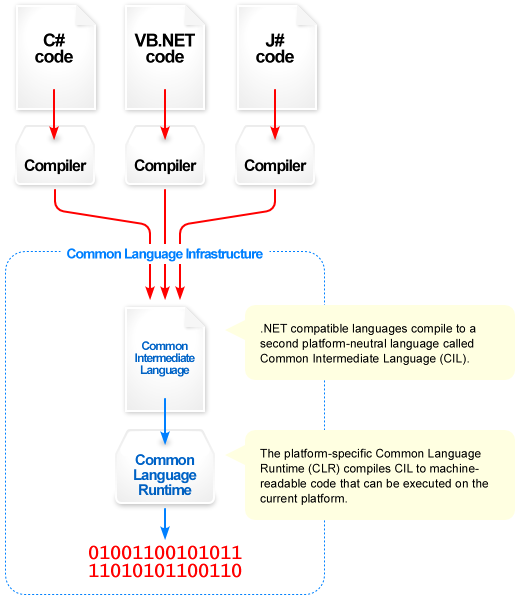
\includegraphics[width=0.85\textwidth]{OverviewOfCLI.png}
	\caption{Overview of the Common Language Infrastructure (CLI) \cite{WikipediaDotNetFramework2007a}.}
	\label{fig:OverviewOfCLI}
\end{figure}
\fi

\if@includefigs@
\begin{figure}[p]
	\centering
	\subfigure[]{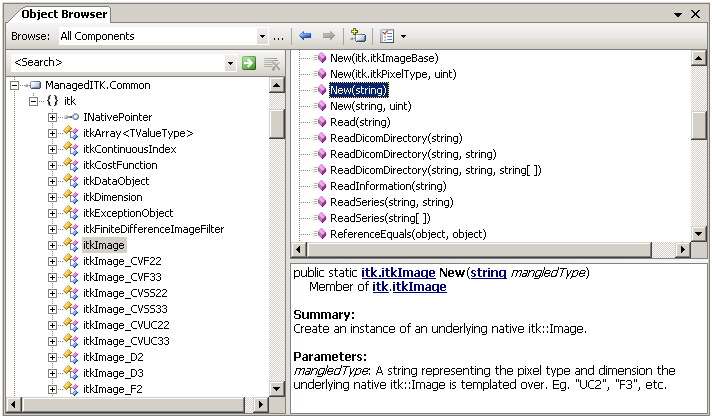
\includegraphics[width=0.90\textwidth]{FeatureObjectBrowser1.png}}
    %\hspace{2.5mm}
    %\subfigure[]{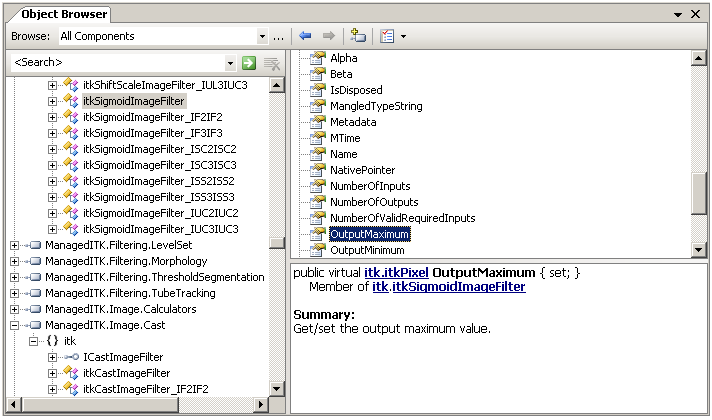
\includegraphics[width=0.90\textwidth]{FeatureObjectBrowser2}}
	\caption{Using the Visual Studio Object Browser.}
	\label{fig:FeatureObjectBrowser}
\end{figure}
\fi

\if@includefigs@
\begin{figure}[p]
	\centering
	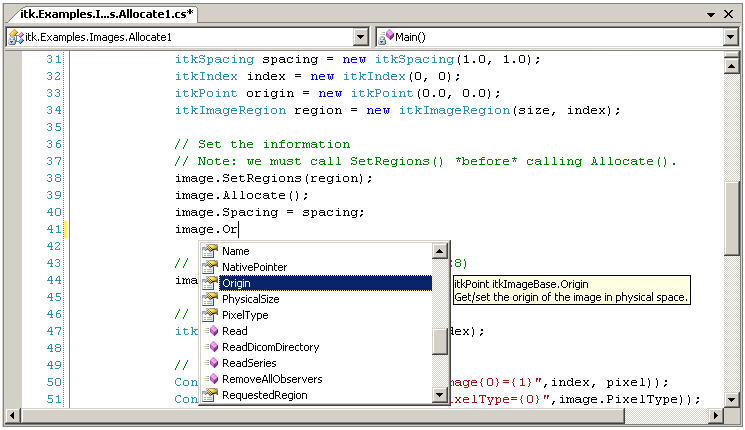
\includegraphics[width=0.90\textwidth]{FeatureAutoComplete1.png}
	\caption{Using Visual Studio Auto-completion.}
	\label{fig:FeatureAutoComplete}
\end{figure}
\fi

%----------------------------------------------------------------------%
% Section
%----------------------------------------------------------------------%
\section{Using ManagedITK}

\subsection{Using the Pre-compiled Assemblies}
\label{sec:UsingPreCompiledAssemblies}
Accompanying this article is the full source-code to compile the
ManagedITK wrappers.
However, unless you need to make changes or additions to the provided assemblies,
it is recommended you use the pre-compiled assemblies.
To use these assemblies in an application, follow these steps:
\begin{enumerate}
	\item Download and unzip the pre-compiled assemblies from: %
			\href{http://insight-journal.org/dspace/handle/1926/501}
			     {The Insight Journal}.
	\item Ensure the .NET Framework 2.0 is installed on your system.
		  See 
\href{http://www.microsoft.com/downloads/details.aspx?familyid=0856EACB-4362-4B0D-8EDD-AAB15C5E04F5}{here} to download the .NET Framework Redistributable Package \code{dotnetfx.exe}.
	\item Install the Microsoft Visual C++ 2005 Redistributable Package
		  \code{vc\_redist\_x86.exe} available from %
		  \href{http://www.microsoft.com/downloads/details.aspx?FamilyID=200B2FD9-AE1A-4A14-984D-389C36F85647}{here}.
		  You may be required to reboot your computer after installing these
		  redistributable libraries.
	\item Open Visual Studio and create a new project eg. a ``Console Application''.
	\item Expand the project in the Solution Explorer, right-click ``References'', and then
			select ``Add References...''.
	\item Select the ``Browse'' tab and browse to the folder where you 
			unzipped the pre-compiled assemblies. 
	\item Select the \code{ManagedITK.Common.dll} assembly and any other required
		    assemblies (use the Ctrl key to select multiple files). Click OK.
	\item You are now ready to use ITK from your .NET project!
\end{enumerate}

\subsection{Compiling the Assemblies}
To compile the ManagedITK assemblies from the source-code with Microsoft Visual Studio 8.0,
follow these steps:
\begin{description}
	\item[1. Download Source:] The latest and greatest source files can be downloaded 
			from: %
			\href{http://insight-journal.org/dspace/handle/1926/501}
			     {The Insight Journal}
	\item[2. Unzip Source:] Unzip the source to a folder, such as\\ \code{C:/Insight-Toolkit/Wrapping/ManagedITK}.
	\item[3. Patch ITK:] Follow the instructions in the \code{Patch} folder to patch your ITK source 
			to fix a bug caused by the Visual Studio 8.0 compiler.			
			Hopefully these patches can be included in the ITK CVS source in the future.
	\item[4. Configure and Build ITK:] 
			Configure and build ITK 3.2.0 or greater with \code{ITK\_USE\_REVIEW = ON}.
	\item[5. Configure ManagedITK:]
			Open CMake and set the source-code to the 
			folder containing the unzipped source and the build path to the desired location
			(as of v3.2.0.2 ManagedITK supports both in-source and out-of-source builds).
			The example projects currently have the build path hard-coded, expecting \code{Buildx86};
			if you chose another location you will have to manually change the references for
			each C\# project under the \code{Examples} folder.
			Click the Configure button and select ``Visual Studio 8 2005''\footnote{
			ManagedITK requires .NET Framework 2.0 or greater. It has only been tested
			using Visual Studio 8.0 2005 (with SP1), however it \emph{should}
			work with Visual C++ 2005 Express Edition.}.
			Set the \code{ITK\_DIR} and \code{WRAP\_*} variables as desired.
			Click the OK button to finish the configuration.		
	\item[6. Convert to Managed Projects:]
			\emph{Before} opening the projects, run the \code{FinishCMake.bat} 
			file located in the build folder.
			Because CMake does not support managed projects,
			this batch file is required to convert the generated \code{vcproj} 
			files into managed projects.
	\item[7. Open Solution:] Open the \code{ManagedITK.sln} solution file. 
			If you have a dual processor or multi-threaded machine,
			set the parallel project build option as desired.
			To configure this feature, go to Tools\textgreater Options\textgreater Projects 
			and Solutions\textgreater Build and Run and type
			the maximum number of parallel builds in the text box.
	\item[8. Build Projects:]
			Build all the projects by right-clicking \code{ALL\_BUILD} and selecting
			\code{Build}.
			The \code{ALL\_BUILD} project automatically builds all the projects
			taking care of dependencies.
\end{description}

%----------------------------------------------------------------------%
% Examples
%----------------------------------------------------------------------%
\section{Examples}

%----------------------------------------------------------------------%
\subsection{Images}

\subsubsection{Allocating an Image}
The source code for this section can be found in the file\\
\code{Examples/Images/itk.Examples.Images.Allocate1.cs}.

This example illustrates how to manually construct and allocate
a managed \code{itk::Image}. 
Firstly, we use the \code{itk} namespace (this step is not necessary but
makes the code more user friendly%
\footnote{The additional \code{itk} at the front of the name of every managed
class was incorporated for two reasons: 1. a similar convention is used for other
wrappings (eg. VTK .NET Wrappers: \href{http://vtkdotnet.sourceforge.net}{http://vtkdotnet.sourceforge.net}), 
and 2. doing so allows both the native and managed versions to be used 
without conflict in languages which support both (eg. C++/CLI).}):
\begin{center}
	\lstset@csharpexample
	\lstinputlisting[linerange={2-2}]
	{../Examples/Images/itk.Examples.Images.Allocate1.cs}
\end{center}

Recall in native ITK, images are templated over the pixel type
and the number of dimensions. Templates are not supported by the CLR,
so ManagedITK explicitly wraps images with different template 
combinations. ManagedITK also includes numerous \emph{wrapper} types,
however this particular example only uses an \emph{explicit} type.
Similar to native ITK, the image is created using 
the \code{New()} method:
\begin{center}
	\lstset@csharpexample
	\lstinputlisting[linerange={25-27}]
	{../Examples/Images/itk.Examples.Images.Allocate1.cs}
\end{center}

Finally, we create and set an image region, \code{Allocate} the memory,
and fill the buffer:
\begin{center}
	\lstset@csharpexample
	\lstinputlisting[linerange={29-29,34-39,42-44}]
	{../Examples/Images/itk.Examples.Images.Allocate1.cs}
\end{center}

Executing the example gives the following output:
\lstset@console
\begin{lstlisting}
> itk.Examples.Images.Allocate1
Image[0, 0]=128
PixelType=Unsigned Char
Dimension=2
Size=[128, 128]
Spacing=[1.0, 1.0]
Origin=[000.00, 000.00]
\end{lstlisting}

\subsubsection{Reading Image Information}
\label{sec:Examples:ReadImageInformation}
The source code for this section can be found in the file\\
\code{Examples/Images/itk.Examples.Images.ReadInformation1.cs}.

The native \code{itk::ImageIOBase::ReadImageInformation()} method
gives applications the ability to peek at the image information 
without unnecessarily reading the image data. A similar static method
is provided by \code{itkImageBase.ReadInformation()}, which
returns an \code{itkImageInformation} structure containing
the number of dimensions, pixel type, size, spacing and origin.
\begin{center}
	\lstset@csharpexample
	\lstinputlisting[linerange={20-21}]
	{../Examples/Images/itk.Examples.Images.ReadInformation1.cs}
\end{center}

The information structure can be used to choose the image type
at \emph{run-time}, as shown in this example:
\begin{center}
	\lstset@csharpexample
	\lstinputlisting[linerange={31-32}]
	{../Examples/Images/itk.Examples.Images.ReadInformation1.cs}
\end{center}

Executing the example gives the following output:
\lstset@console
\begin{lstlisting}
> itk.Examples.Images.ReadInformation1 cthead1.png
Information --------------------------
PixelType=RGB Unsigned Char
Dimension=2
Size=[256, 256]
Spacing=[1.0, 1.0]
Origin=[000.00, 000.00]
Image --------------------------------
Name=cthead1.png
PixelType=RGB Unsigned Char
Dimension=2
Size=[256, 256]
Spacing=[1.0, 1.0]
Origin=[000.00, 000.00]
Buffer=57064620
\end{lstlisting}


\subsubsection{Reading and Writing Images}
The source code for this section can be found in the file\\
\code{Examples/Images/itk.Examples.Images.ReadWrite1.cs}.

One of the benefits of ManagedITK is the ability to easily
choose the image type at \emph{run-time}, rather than compile-time.
This example shows how to read and write an image, using a command line
argument to determine the type at run-time.

Firstly, we use the \code{itk} namespace:
\begin{center}
	\lstset@csharpexample
	\lstinputlisting[linerange={2-2}]
	{../Examples/Images/itk.Examples.Images.ReadWrite1.cs}
\end{center}

Next, we use a command line string argument (such as \code{"UC2"} or \code{"IF3"})
to instantiate an image:
\begin{center}
	\lstset@csharpexample
	\lstinputlisting[linerange={20-21}]
	{../Examples/Images/itk.Examples.Images.ReadWrite1.cs}
\end{center}

For sake of ease the \code{itk::ImageFileReader}, \code{itk::ImageFileWriter},
and other associated objects have been directly incorporated into
the managed \code{itkImage} class. This means that image IO can be accomplished
very easily only using the image object.
Note that the underlying native \code{itk::Image} is not actually created until
a call to one of the following methods is made: \code{Read()}, \code{ReadSeries()}, 
\code{ReadDicomDirectory()}, or \code{Allocate()}. 
The \code{Read()} method takes a single \code{String} argument for the input file name:
\begin{center}
	\lstset@csharpexample
	\lstinputlisting[linerange={23-24}]
	{../Examples/Images/itk.Examples.Images.ReadWrite1.cs}
\end{center}

Similarly the \code{Write()} method takes a single \code{String} argument for the output file name:
\begin{center}
	\lstset@csharpexample
	\lstinputlisting[linerange={35-36},]
	{../Examples/Images/itk.Examples.Images.ReadWrite1.cs}
\end{center}

Executing the example gives the following output:
\lstset@console
\begin{lstlisting}
> itk.Examples.Images.ReadWrite1 "F2" cthead1.png cthead1_OUT.mhd
Name=cthead1.png
PixelType=Float
Dimension=2
Size=[256, 256]
Spacing=[1.0, 1.0]
Origin=[000.00, 000.00]
Buffer=57065616
\end{lstlisting}


\subsubsection{Reading DICOM Images}
The source code for this section can be found in the file\\
\code{Examples/Images/itk.Examples.Images.ReadDicom1.cs}.

The \code{itkImageBase.ReadDicomDirectory()} method uses the 
native \code{itk::GDCMImageIO} to read an image from a DICOM directory.
As discussed in the previous example, calling this method creates
the underlying native \code{itk::Image}.
The \code{ReadDicomDirectory()} method expects a \code{String} specifying
the directory, however overrides also exist allowing you to specify the
series id and/or restrictions.

In this example we are expecting the DICOM directory to hold
a 3D scalar image with \code{SignedShort} component type:
\begin{center}
	\lstset@csharpexample
	\lstinputlisting[linerange={16-17}]
	{../Examples/Images/itk.Examples.Images.ReadDicom1.cs}
\end{center}

The DICOM directory is passed in via a command line argument:
\begin{center}
	\lstset@csharpexample
	\lstinputlisting[linerange={19-20}]
	{../Examples/Images/itk.Examples.Images.ReadDicom1.cs}
\end{center}

Finally, the extracted image can be saved in a different format:
I recommend the MetaImage format (*.mhd):
\begin{center}
	\lstset@csharpexample
	\lstinputlisting[linerange={31-32}]
	{../Examples/Images/itk.Examples.Images.ReadDicom1.cs}
\end{center}

We have not included a DICOM series in the examples, however executing
the example with an appropriate directory gives the following output:
\lstset@console
\begin{lstlisting}
> itk.Examples.Images.ReadDicom1 D:\AA1\AA1\AA12345 C:\Temp\AA12456.mhd
Name=D:\AA1\AA1\AA12345
PixelType=Signed Short
Dimension=3
Size=[144, 144, 234]
Spacing=[4.0, 4.0, 4.0]
Origin=[-286.59, -216.59, -1041.35]
Buffer=66715680
\end{lstlisting}

\subsubsection{Reading and Writing Image Series}
The source code for this section can be found in the file\\
\code{Examples/Images/itk.Examples.Images.ReadWriteSeries1.cs}.

This example explains the usage of the \code{itkImageBase.ReadSeries()} and
\code{itkImageBase.WriteSeries()} methods.

The \code{itkImageBase.ReadSeries()} method expects an array of file names.
Alternatively it expects a base path and a file name
containing the wildcard character `\code{*}' (referred to as a \emph{pattern}).
An example for the pattern argument might be: \code{myfilename*.png}.
\begin{center}
	\lstset@csharpexample
	\lstinputlisting[linerange={19-19,21-21}]
	{../Examples/Images/itk.Examples.Images.ReadWriteSeries1.cs}
\end{center}

The \code{itkImageBase.WriteSeries()} method expects a file name format,
with the `\code{\{0\}}' string. This format placeholder is replaced with
the series id or slice number. The format of the series id can also be
specified: for example \code{"000"} forces the series id to have at least
three digits. Any numeric format string supported by \code{Int32.ToString()}
can be passed in as the series id format.
\begin{center}
	\lstset@csharpexample
	\lstinputlisting[linerange={31-31,34-34}]
	{../Examples/Images/itk.Examples.Images.ReadWriteSeries1.cs}
\end{center}

Executing the example with 
\code{a7b1.jpg}, 
\code{a7b2.jpg}, 
\code{a7b3.jpg}, and 
\code{a7b4.jpg} in the path \code{C:/itk} gives the following output:
\lstset@console
\begin{lstlisting}
>itk.Examples.Images.ReadWriteSeries1 "C:/itk" "a7b*.png" "a7c{0}.jpg" "00"
PixelType=Unsigned Char
Dimension=3
Size=[72, 72, 4]
Spacing=[1.0, 1.0, 1.0]
Origin=[000.00, 000.00, 000.00]
Buffer=57044976
\end{lstlisting}

and writes the files: 
\code{a7c00.jpg}, 
\code{a7c01.jpg}, 
\code{a7c02.jpg}, and 
\code{a7c03.jpg}.

\subsubsection{Displaying images using System.Drawing.Bitmap}
\label{sec:Examples:Bitmap1}
The source code for this section can be found in the file\\
\code{Examples/Images/itk.Examples.Images.FormBitmap1.cs}.

This example shows how to use ManagedITK with \code{System.Drawing.Bitmap}.
It should be noted that the \code{System.Drawing} namespace is a managed wrapper
around the Windows GDI+ library, and as such only supports 8-bit images 
(which is far from ideal for medical imaging applications).
ManagedITK can be used to perform operations on images with a pixel depth
greater than 8-bits, however only 8-bit images can be displayed using 
\code{System.Drawing.Bitmap}\footnote{OpenGL supports a much broader range of pixel types.
Tao is a .NET binding around the OpenGL library suitable for use with ManagedITK: 
\href{http://taoframework.com}{http://taoframework.com}.}. 

To display an \code{itkImageBase} using the \code{System.Drawing} namespace
we must firstly use the required assemblies:
\begin{center}
	\lstset@csharpexample
	\lstinputlisting[linerange={2-4,6-6}]
	{../Examples/Images/itk.Examples.Images.FormBitmap1.cs}
\end{center}

Next, we create and read a 2D 8-bit scalar image:
\begin{center}
	\lstset@csharpexample
	\lstinputlisting[linerange={26-28}]
	{../Examples/Images/itk.Examples.Images.FormBitmap1.cs}
\end{center}

Next, we set the pixel format to support 8-bit grayscale images:
\begin{center}
	\lstset@csharpexample
	\lstinputlisting[linerange={82-83}]
	{../Examples/Images/itk.Examples.Images.FormBitmap1.cs}
\end{center}

The data in \code{Bitmap} objects are not tightly packed,
rows of bytes are stored in multiples of four (the multiple-four width of 
an image known as the \emph{stride}).
If the width and stride are not equal, we must perform some non-trivial
operations to copy the image buffer into the \code{Bitmap}. However,
if the width and stride are equal, we can simply use the \code{Bitmap}
constructor%
\footnote{The method described in this example uses the 
\code{itk::Image::GetBufferPointer()}.
This is not an ideal solution and --- from discussions on the
\code{insight-developers} mailing list ---
can not be guaranteed to exist in the future.
Making this method public has been considered poor design
because it forces the \code{itk::Image} to store data in a
contiguous array.
However, for the moment it remains a suitable means to obtain
the image data.}:
\begin{center}
	\lstset@csharpexample
	\lstinputlisting[linerange={88-94}]
	{../Examples/Images/itk.Examples.Images.FormBitmap1.cs}
\end{center}

Finally, we set the \code{Bitmap.Palette}:
\begin{center}
	\lstset@csharpexample
	\lstinputlisting[linerange={124-125}]
	{../Examples/Images/itk.Examples.Images.FormBitmap1.cs}
\end{center}

Executing the example as below opens the window shown in Figure~\ref{fig:ExamplesImagesBitmap1a}:
\lstset@console
\begin{lstlisting}
> itk.Examples.Images.Bitmap1 cthead1.png
\end{lstlisting}

\if@includefigs@
\begin{figure}
	\centering
	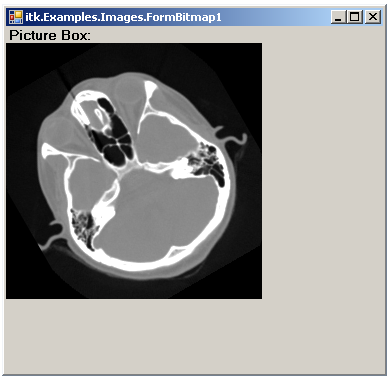
\includegraphics[width=250pt]{itkExamplesImagesBitmap1.png}
	\caption{Output from \code{Examples/Images/itk.Examples.Images.Bitmap1.cs}.}
	\label{fig:ExamplesImagesBitmap1a}
\end{figure}
\fi


%----------------------------------------------------------------------%
\subsection{Iterators}
The source code for this section can be found in the file\\
\code{Examples/Iterators/itk.Examples.Iterators.ImageRegionIterator1.cs}.

This example shows how to use an \code{ImageRegionIterator} to iterate over
the each pixel in an image. The interesting aspect to note is the use
of the \code{foreach} syntax.

We begin by creating and reading an image using an explicit type:
\begin{center}
	\lstset@csharpexample
	\lstinputlisting[linerange={17-19}]
	{../Examples/Iterators/itk.Examples.Iterators.ImageRegionIterator1.cs}
\end{center}

Next, we allocate an empty image for the output:
\begin{center}
	\lstset@csharpexample
	\lstinputlisting[linerange={21-27}]
	{../Examples/Iterators/itk.Examples.Iterators.ImageRegionIterator1.cs}
\end{center}

Next, we create two iterators, one to walk the input image and one to walk 
the output image. Note that iterators are created using the normal C\# \code{new}
command, this is because the native ITK iterators are not derived from 
\code{itk::SmartPointer} and do not use the factory method of instantiation. 
\begin{center}
	\lstset@csharpexample
	\lstinputlisting[linerange={30-34}]
	{../Examples/Iterators/itk.Examples.Iterators.ImageRegionIterator1.cs}
\end{center}

We now walk over both images, setting the output value as the input value.
Note the use of the \code{foreach} statement: ManagedITK iterators implement
the \code{System.IEnumerable} interface allowing us to use this syntax
(alternatively a simple \code{for} loop could have been used).
Also note that the \code{foreach} statement can only be used on \emph{one}
iterator, so we must remember to increment any other iterators manually:
\begin{center}
	\lstset@csharpexample
	\lstinputlisting[linerange={36-41}]
	{../Examples/Iterators/itk.Examples.Iterators.ImageRegionIterator1.cs}
\end{center}

This example can be executing using the following code to copy the input image:
\lstset@console
\begin{lstlisting}
> itk.Examples.Iterators.ImageRegionIterator1 cthead1.png cthead1_COPY.png
\end{lstlisting}

%----------------------------------------------------------------------%
\subsection{Filters}

\subsubsection{Gradient Magnitude}
The source code for this section can be found in the file\\
\code{Examples/Filters/itk.Examples.Filters.GradientMagnitude1.cs}.

This example introduces how to use \code{itkImageToImageFilter} objects, 
with the \code{itkGradientMagnitudeImageFilter} as a simple case study.
The most important difference has to do with the \code{itkImageSource.GetOutput()}
method.

Firstly, as usual, we use the \code{itk} namespace:
\begin{center}
	\lstset@csharpexample
	\lstinputlisting[linerange={2-2}]
	{../Examples/Filters/itk.Examples.Filters.GradientMagnitude1.cs}
\end{center}

For code clarity we can define an alias for the \code{itk\-Gradient\-Magnitude\-ImageFilter}:
\begin{center}
	\lstset@csharpexample
	\lstinputlisting[linerange={4-4}]
	{../Examples/Filters/itk.Examples.Filters.GradientMagnitude1.cs}
\end{center}

Next, we create our input and output images, using the command line to specify the type.
Note that we have used the \code{itkImageBase.New(itkImageBase image)} method for the output
image, which creates an explicit type the same as the given image:
\begin{center}
	\lstset@csharpexample
	\lstinputlisting[linerange={18-20}]
	{../Examples/Filters/itk.Examples.Filters.GradientMagnitude1.cs}
\end{center}

Next, we read the input image:
\begin{center}
	\lstset@csharpexample
	\lstinputlisting[linerange={22-23}]
	{../Examples/Filters/itk.Examples.Filters.GradientMagnitude1.cs}
\end{center}

Creating and applying the filter is similar to native ITK, except the template arguments
are moved to the \code{New()} method. In the case below, we have specified the type
parameters as \code{input, output}. This creates the filter type by appending the 
\code{itkObject.ManagedTypeString} from all type parameters: 
eg. \code{"IUC2" + "IUC2" = "IUC2IUC2"}:
\begin{center}
	\lstset@csharpexample
	\lstinputlisting[linerange={25-28}]
	{../Examples/Filters/itk.Examples.Filters.GradientMagnitude1.cs}
\end{center}

If  the template parameters we specify do not create a valid \code{ManagedTypeString}
when appended together, we would receive an exception similar to below:
\lstset@console
\begin{lstlisting}
itk.itkInvalidWrappedTypeException: Could not create an instance of
'itk.itkGradientMagnitudeImageFilter_IUC2'. The given type may not be supported
or may be invalid. 
---> System.NullReferenceException:
The type 'itk.itkGradientMagnitudeImageFilter_IUC2' could not be found in
ManagedITK.Filtering.Common, Version=0.0.0.0, Culture=neutral
   at itk.itkGradientMagnitudeImageFilter.New(String mangledType)
   --- End of inner exception stack trace ---
   at itk.itkGradientMagnitudeImageFilter.New(String mangledType)
   at itk.itkGradientMagnitudeImageFilter.New(INativePointer[] types)
   at itk.Examples.Filters.GradientMagnitude1.Main(String[] args)
      in itk.Examples.Filters.GradientMagnitude1.cs:line 26
\end{lstlisting}

Finally, we retrieve the output by calling \code{itkImageSource.GetOutput()}
with the \code{output} object (the object is required to specify the managed type).
We could also use the \code{GetOutput()} method which returns an \code{IntPtr} to
the native type, but this is of little use in the current example.
\begin{center}
	\lstset@csharpexample
	\lstinputlisting[linerange={29-29}]
	{../Examples/Filters/itk.Examples.Filters.GradientMagnitude1.cs}
\end{center}

Executing the example as below gives the output shown in Figure~\ref{fig:ExamplesFiltersGradientMagnitude1a}:
\lstset@console
\begin{lstlisting}
> itk.Examples.Filters.GradientMagnitude1 UC2 cthead1.png cthead1_G.png
\end{lstlisting}

\if@includefigs@
\begin{figure}
	\centering
	\subfigure[Input]{
		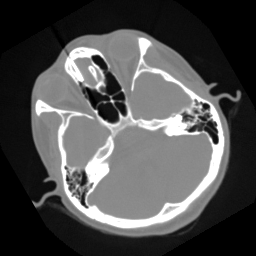
\includegraphics[width=0.4\textwidth]{itkExamplesFiltersGradientMagnitude1Input.png}
	}
    \hspace{2.5mm}
    \subfigure[Output]{
    	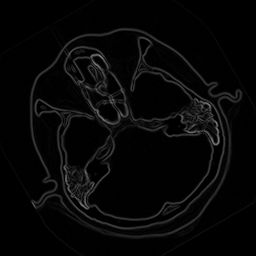
\includegraphics[width=0.4\textwidth]{itkExamplesFiltersGradientMagnitude1Output.png}
    }
    \caption{Output from \code{itk.Examples.Filters.GradientMagnitude1.cs}.}
	\label{fig:ExamplesFiltersGradientMagnitude1a}
\end{figure}
\fi

\subsubsection{Sigmoid (and Managed Events)}
\label{sec:Examples:Sigmoid1}
The source code for this section can be found in the file\\
\code{Examples/Filters/itk.Examples.Filters.Sigmoid1.cs}.

This example demonstrates how to observe native ITK events
using managed events and \code{delegates} 
(the managed type-safe equivalent of C-style function pointers).

We firstly create the input and output images, reading the desired type from the 
command line:
\begin{center}
	\lstset@csharpexample
	\lstinputlisting[linerange={19-21}]
	{../Examples/Filters/itk.Examples.Filters.Sigmoid1.cs}
\end{center}

Next, we read the input image from disk:
\begin{center}
	\lstset@csharpexample
	\lstinputlisting[linerange={23-25}]
	{../Examples/Filters/itk.Examples.Filters.Sigmoid1.cs}
\end{center}

Now we create the filter, and set the input, output and filter parameters:
\begin{center}
	\lstset@csharpexample
	\lstinputlisting[linerange={26-34}]
	{../Examples/Filters/itk.Examples.Filters.Sigmoid1.cs}
\end{center}

In the code block above note how we add observers to the 
\code{Started}, \code{Progress}, and \code{Ended} events.
To observe an event, we simply create a \code{delegate}
which references a function containing the desired logic
for the event. For example, in the \code{Started} event
handler we print out a string to the console with the
time the filter started:
\begin{center}
	\lstset@csharpexample
	\lstinputlisting[linerange={51-56}]
	{../Examples/Filters/itk.Examples.Filters.Sigmoid1.cs}
\end{center}

Finally we write the output to disk. Note that the \code{Write}
method will automatically update any upstream filters:
\begin{center}
	\lstset@csharpexample
	\lstinputlisting[linerange={37-37,39-39}]
	{../Examples/Filters/itk.Examples.Filters.Sigmoid1.cs}
\end{center}

Executing the example as below gives the following output:
\lstset@console
\begin{lstlisting}
>itk.Examples.Filters.Sigmoid1 UC2 cthead1.png -60.0 90.0 cthead1_SIGMOID.png
itk.itkSigmoidImageFilter: Started at 19/01/2007 10:16:03 AM
001% 002% 003% 004% 005% 006% 007% 008% 009% 010%
011% 012% 013% 014% 015% 016% 017% 018% 019% 020%
021% 022% 023% 024% 025% 026% 027% 028% 029% 030%
031% 032% 033% 034% 035% 036% 037% 038% 039% 040%
041% 042% 043% 044% 045% 046% 047% 048% 049% 050%
051% 052% 053% 054% 055% 056% 057% 058% 059% 060%
061% 062% 063% 064% 065% 066% 067% 068% 069% 070%
071% 072% 073% 074% 075% 076% 077% 078% 079% 080%
081% 082% 083% 084% 085% 086% 087% 088% 089% 090%
091% 092% 093% 094% 095% 096% 097% 098% 099% 100%
itk.itkSigmoidImageFilter: Ended at 19/01/2007 10:16:03 AM
\end{lstlisting}


\subsection{Segmentation}

\subsubsection{Binary Threshold (and Simple GUI)}
\label{sec:Examples:BinaryThreshold1}
The source code for this section can be found in the file\\
\code{Examples/Filters/itk.Examples.Segmentation.FormBinaryThreshold1.cs}.

This example shows how to use the \code{itkBinaryThresholdImageFilter}.
In addition is shows how to use \code{System.Windows.Forms} to control and
monitor a filter which is running on a separate thread.

Firstly we use various namespaces:
\begin{center}
	\lstset@csharpexample
	\lstinputlisting[linerange={1-5}]
	{../Examples/Segmentation/itk.Examples.Segmentation.FormBinaryThreshold1.cs}
\end{center}

For sake of ease we introduce a type alias:
\begin{center}
	\lstset@csharpexample
	\lstinputlisting[linerange={7-7}]
	{../Examples/Segmentation/itk.Examples.Segmentation.FormBinaryThreshold1.cs}
\end{center}

Using the Visual Studio Windows Designer, we create a \code{Form} with a 
menu containing two items: ``Open'' and ``Exit''. When the user clicks the 
``Open'' menu item, the user will be prompted for an image file name:
\begin{center}
	\lstset@csharpexample
	\lstinputlisting[linerange={25-42}]
	{../Examples/Segmentation/itk.Examples.Segmentation.FormBinaryThreshold1.cs}
\end{center}

If the user selects a valid file name and clicks ``OK'', the processing thread will start:
\begin{center}
	\lstset@csharpexample
	\lstinputlisting[linerange={48-52}]
	{../Examples/Segmentation/itk.Examples.Segmentation.FormBinaryThreshold1.cs}
\end{center}

In the new thread, we firstly determine the image information and create
input and output images:
\begin{center}
	\lstset@csharpexample
	\lstinputlisting[linerange={79-82}]
	{../Examples/Segmentation/itk.Examples.Segmentation.FormBinaryThreshold1.cs}
\end{center}

After reading the input image, the filter is started:
\begin{center}
	\lstset@csharpexample
	\lstinputlisting[linerange={88-99}]
	{../Examples/Segmentation/itk.Examples.Segmentation.FormBinaryThreshold1.cs}
\end{center}

The \code{Started}, \code{Progress}, and \code{Ended} events are observed with
thread-safe methods which update the GUI as the filter is running. For example,
the progress observer increments a \code{ProgressBar}:
\begin{center}
	\lstset@csharpexample
	\lstinputlisting[linerange={144-156}]
	{../Examples/Segmentation/itk.Examples.Segmentation.FormBinaryThreshold1.cs}
\end{center}

Executing the example as below gives the output shown in Figure~\ref{fig:ExamplesSegmentationBinaryThreshold1a}:

\lstset@console
\begin{lstlisting}
>itk.Examples.Segmentation.BinaryThreshold1
\end{lstlisting}

\if@includefigs@
\begin{figure}
	\centering
	\subfigure[Screen shot]{
		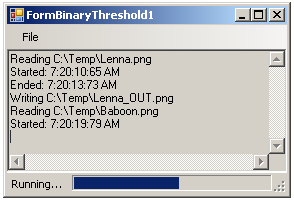
\includegraphics[width=0.45\textwidth]{itkExamplesSegmentationBinaryThreshold1Screen.png}
	}
    \hspace{3.0cm}
	\subfigure[Input]{
		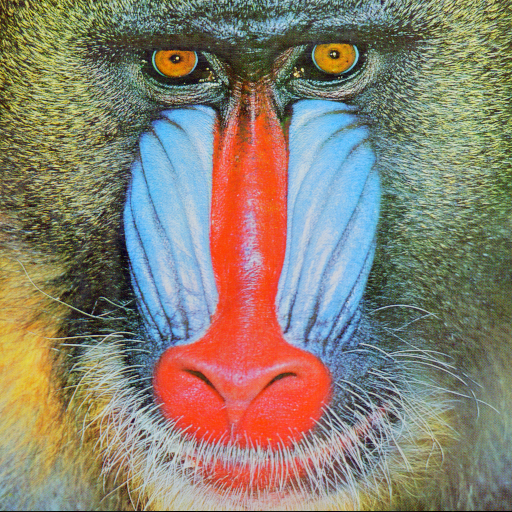
\includegraphics[width=0.35\textwidth]{itkExamplesSegmentationBinaryThreshold1Input.png}
	}
    \hspace{0.25mm}
    \subfigure[Output]{
    	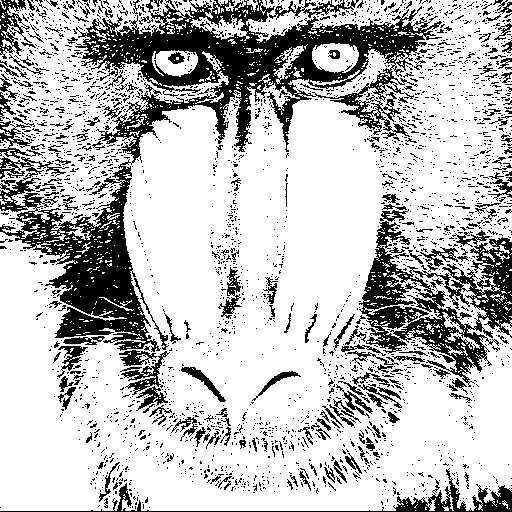
\includegraphics[width=0.35\textwidth]{itkExamplesSegmentationBinaryThreshold1Output.png}
    }
    \caption{Output from \code{itk.Examples.Segmentation.BinaryThreshold1.cs}.}
	\label{fig:ExamplesSegmentationBinaryThreshold1a}
\end{figure}
\fi

\subsubsection{Watershed (and Pipeline)}
The source code for this section can be found in the file\\
\code{Examples/Segmentation/itk.Examples.Segmentation.Watershed1.cs}.

This example shows how to use the \code{itkWatershedImageFilter}.
It also demonstrates the usage of a pipeline.

Firstly, we use the \code{itk} namespace and in addition we create
some aliases for code clarity:
\begin{center}
	\lstset@csharpexample
	\lstinputlisting[linerange={2-7}]
	{../Examples/Segmentation/itk.Examples.Segmentation.Watershed1.cs}
\end{center}

Next, we create the input and output label images:
\begin{center}
	\lstset@csharpexample
	\lstinputlisting[linerange={22-25}]
	{../Examples/Segmentation/itk.Examples.Segmentation.Watershed1.cs}
\end{center}

We now set up the watershed filter, noting that its \code{New()} method
only expects a single type argument:
\begin{center}
	\lstset@csharpexample
	\lstinputlisting[linerange={27-32}]
	{../Examples/Segmentation/itk.Examples.Segmentation.Watershed1.cs}
\end{center}

Finally, we connect the filter output to a relabeller using similar
syntax as native ITK:
\begin{center}
	\lstset@csharpexample
	\lstinputlisting[linerange={34-38}]
	{../Examples/Segmentation/itk.Examples.Segmentation.Watershed1.cs}
\end{center}

Executing the example as below gives the output shown in Figure~\ref{fig:ExamplesSegmentationWatershed1a}:
\lstset@console
\begin{lstlisting}
>itk.Examples.Segmentation.Watershed1 UC2 cthead1.png 0.3 0.22 
 cthead1_WATERSHED.mhd
\end{lstlisting}

\if@includefigs@
\begin{figure}
	\centering
	\subfigure[Input]{
		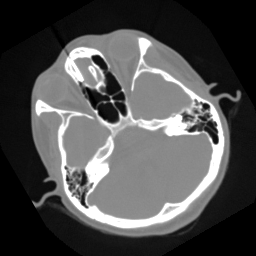
\includegraphics[width=0.3\textwidth]{itkExamplesSegmentationWatershed1Input.png}
	}
    \hspace{0.25mm}
	\subfigure[Coloured Output]{
		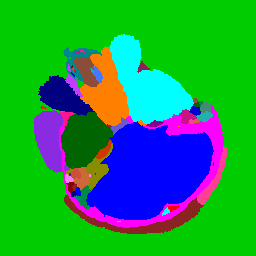
\includegraphics[width=0.3\textwidth]{itkExamplesSegmentationWatershed1Output.png}
	}
    \hspace{0.25mm}
    \subfigure[Coloured Overlay]{
    	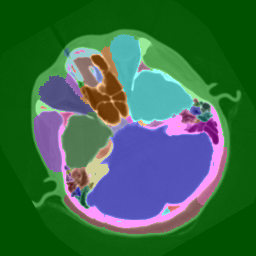
\includegraphics[width=0.3\textwidth]{itkExamplesSegmentationWatershed1Overlay.png}
    }
    \caption{Output from \code{itk.Examples.Segmentation.Watershed1.cs}.}
	\label{fig:ExamplesSegmentationWatershed1a}
\end{figure}
\fi

\subsubsection{Level Set Segmentation}
The source code for this section can be found in the file\\
\code{Examples/Segmentation/itk.Examples.Segmentation.LevelSet1.cs}.

This example shows how to use the \code{itkCurvesLevelSetImageFilter}.

Firstly, we create an alias for code clarity:
\begin{center}
	\lstset@csharpexample
	\lstinputlisting[linerange={4-4}]
	{../Examples/Segmentation/itk.Examples.Segmentation.LevelSet1.cs}
\end{center}

Next, we create the initial, speed, and output images by reading the 
dimensionality from the command line:
\begin{center}
	\lstset@csharpexample
	\lstinputlisting[linerange={18-27}]
	{../Examples/Segmentation/itk.Examples.Segmentation.LevelSet1.cs}
\end{center}

We now create and set up the \code{itkCurvesLevelSetImageFilter}:
\begin{center}
	\lstset@csharpexample
	\lstinputlisting[linerange={29-43}]
	{../Examples/Segmentation/itk.Examples.Segmentation.LevelSet1.cs}
\end{center}

We watch for the \code{Started}, \code{Iteration}, and \code{Ended} events.
For the iteration event, we write out the number of elapsed iteration
in a nice block format:
\begin{center}
	\lstset@csharpexample
	\lstinputlisting[linerange={61-69}]
	{../Examples/Segmentation/itk.Examples.Segmentation.LevelSet1.cs}
\end{center}

Finally, we write the output:
\begin{center}
	\lstset@csharpexample
	\lstinputlisting[linerange={45-47}]
	{../Examples/Segmentation/itk.Examples.Segmentation.LevelSet1.cs}
\end{center}

Executing the example as below gives the output shown in Figure~\ref{fig:ExamplesSegmentationLevelSet1a}:

\lstset@console
\begin{lstlisting}
>itk.Examples.Segmentation.LevelSet1 2 BrainProtonDensitySlice_INITIAL.mhd 
 BrainProtonDensitySlice_SPEED.mhd BrainProtonDensitySlice_LEVELSET.mhd
Reading initial: BrainProtonDensitySlice_INITIAL.mhd
Reading feature: BrainProtonDensitySlice_SPEED.mhd
Started: 4/04/2007 9:47:19 AM
001 010 020 030 040 050 060 070 080 090
100 110 120 130 140 150 160 170 180 190
200 210 220 230 240 250 260 270 280 290
300 310 320 330 340 350 360 370 380 390
400 410 420 430 440 450 460 470 480 490
500 510 520 530 540 550 560 570 580 590
600
Ended: 4/04/2007 9:47:20 AM
Writing output: BrainProtonDensitySlice_LEVELSET.mhd
\end{lstlisting}

\if@includefigs@
\begin{figure}
	\centering
	\subfigure[Initial]{
		
\includegraphics[width=0.28\textwidth]{itkExamplesSegmentationLevelSet1Initial.png}
	}
    \hspace{0.25mm}
	\subfigure[Speed]{
		
\includegraphics[width=0.28\textwidth]{itkExamplesSegmentationLevelSet1Speed.png}
	}
    \hspace{0.25mm}
    \subfigure[Final]{
    	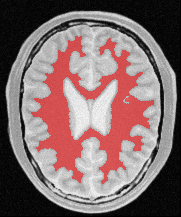
\includegraphics[width=0.28\textwidth]{itkExamplesSegmentationLevelSet1Overlay.png}
    }
    \hspace{2.0cm}
    \vspace{1.0cm}
    \subfigure[0 iterations]{
    	
\includegraphics[width=0.14\textwidth]{itkExamplesSegmentationLevelSet1_000.png}
    }
    \hspace{0.25mm}
    \subfigure[50 iterations]{
    	
\includegraphics[width=0.14\textwidth]{itkExamplesSegmentationLevelSet1_050.png}
    }
    \hspace{0.25mm}
    \subfigure[100 iterations]{
    	
\includegraphics[width=0.14\textwidth]{itkExamplesSegmentationLevelSet1_100.png}
    }
    \hspace{0.25mm}
    \subfigure[150 iterations]{
    	
\includegraphics[width=0.14\textwidth]{itkExamplesSegmentationLevelSet1_150.png}
    }
    \hspace{0.25mm}
    \subfigure[200 iterations]{
    	
\includegraphics[width=0.14\textwidth]{itkExamplesSegmentationLevelSet1_200.png}
    }
    \hspace{0.25mm}
    \subfigure[250 iterations]{
    	
\includegraphics[width=0.14\textwidth]{itkExamplesSegmentationLevelSet1_250.png}
    }
    \caption{Output from \code{itk.Examples.Segmentation.LevelSet1.cs}.}
	\label{fig:ExamplesSegmentationLevelSet1a}
\end{figure}
\fi


%----------------------------------------------------------------------%
\subsection{Registration}
The source code for this section can be found in the file\\
\code{Examples/Registration/itk.Examples.Registration.Translation1.cs}.

This example shows how to use the Registration wrappers.
It requires four different assemblies:
\code{ManagedITK.Common.dll},
\code{ManagedITK.Interpolators.dll},
\code{ManagedITK.Registration.dll}, and
\code{ManagedITK.Transform.dll}.

Firstly, we use the \code{itk} namespace and define some aliases:
\begin{center}
	\lstset@csharpexample
	\lstinputlisting[linerange={3-11}]
	{../Examples/Registration/itk.Examples.Registration.Translation1.cs}
\end{center}

Next, we read the fixed image from the command line:
\begin{center}
	\lstset@csharpexample
	\lstinputlisting[linerange={25-27}]
	{../Examples/Registration/itk.Examples.Registration.Translation1.cs}
\end{center}

We now construct a moving image by translating the fixed image by a 
known amount:
\begin{center}
	\lstset@csharpexample
	\lstinputlisting[linerange={29-30,33-33,36-37,42-49}]
	{../Examples/Registration/itk.Examples.Registration.Translation1.cs}
\end{center}

Next, we set up the metric and optimizer (the optimizer values were
taken from the ITK Software Guide):
\begin{center}
	\lstset@csharpexample
	\lstinputlisting[linerange={60-68}]
	{../Examples/Registration/itk.Examples.Registration.Translation1.cs}
\end{center}

Note that we add an observer to the optimizer \code{Iteration} event:
\begin{center}
	\lstset@csharpexample
	\lstinputlisting[linerange={101-108}]
	{../Examples/Registration/itk.Examples.Registration.Translation1.cs}
\end{center}

Finally, we plug everything together and start the registration algorithm:
\begin{center}
	\lstset@csharpexample
	\lstinputlisting[linerange={70-79}]
	{../Examples/Registration/itk.Examples.Registration.Translation1.cs}
\end{center}

Executing the example as below gives the output shown in Figure~\ref{fig:ExamplesRegistrationTranslation1a}:

\lstset@console
\begin{lstlisting}
>itk.Examples.Registration.Translation1 cthead1.png
START: [007.50, 012.00]
000:   [008.20, 008.06]
001:   [005.34, 005.28]
002:   [002.74, 002.23]
003:   [001.32, -001.51]
004:   [-001.14, -004.66]
005:   [-003.17, -008.11]
006:   [-006.29, -010.61]
007:   [-008.82, -013.71]
008:   [-007.60, -012.13]
009:   [-005.97, -010.97]
010:   [-006.83, -011.48]
011:   [-007.63, -012.08]
012:   [-007.15, -011.93]
013:   [-007.40, -011.94]
014:   [-007.64, -012.00]
015:   [-007.52, -012.01]
016:   [-007.40, -012.01]
017:   [-007.46, -012.00]
018:   [-007.52, -011.99]
019:   [-007.49, -012.00]
020:   [-007.50, -012.00]
END:   [-007.50, -012.00]
\end{lstlisting}

\if@includefigs@
\begin{figure}
	\centering
	\subfigure[Fixed]{
		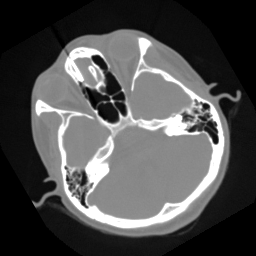
\includegraphics[width=0.3\textwidth]{itkExamplesRegistrationTranslation1Fixed.png}
	}
    \hspace{0.25mm}
	\subfigure[Fixed minus Moving]{
		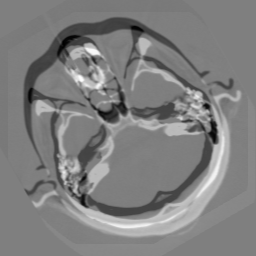
\includegraphics[width=0.3\textwidth]{itkExamplesRegistrationTranslation1FixedSubMoving.png}
	}
    \hspace{0.25mm}
    \subfigure[Fixed minus Result]{
    	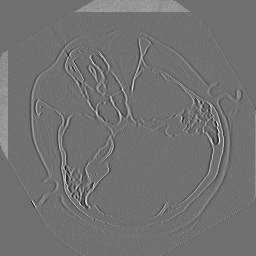
\includegraphics[width=0.3\textwidth]{itkExamplesRegistrationTranslation1FixedSubResult.png}
    }
    \caption{Output from \code{itk.Examples.Registration.Translation1.cs}.}
	\label{fig:ExamplesRegistrationTranslation1a}
\end{figure}
\fi

%----------------------------------------------------------------------%
\subsection{Meshes}
The source code for this section can be found in the file\\
\code{Examples/Meshes/itk.Examples.Meshes.TriangleMesh1.cs}.

This example shows how to convert a triangle mesh to a binary image.

Firstly, we declare some typedefs for use with meshes:
\begin{center}
	\lstset@csharpexample
	\lstinputlisting[linerange={16-19}]
	{../Examples/Meshes/itk.Examples.Meshes.TriangleMesh1.cs}
\end{center}

Next, we use \code{itkRegularSphereMeshSource} to programmatically create a mesh.
Notice that the traits object is passed to the mesh \code{New()} method:
\begin{center}
	\lstset@csharpexample
	\lstinputlisting[linerange={21-29}]
	{../Examples/Meshes/itk.Examples.Meshes.TriangleMesh1.cs}
\end{center}

Finally, we convert the mesh to an image using
\code{itkTriangleMeshToBinaryImageFilter}:
\begin{center}
	\lstset@csharpexample
	\lstinputlisting[linerange={31-39}]
	{../Examples/Meshes/itk.Examples.Meshes.TriangleMesh1.cs}
\end{center}

%----------------------------------------------------------------------%
\subsection{IronPython}
The source code for this section can be found in the file\\
\code{Examples/IronPython/IronPythonSpeedImage1.cs}.

This example simply demonstrates that ManagedITK can be used
by any language which targets the .NET CLR, including IronPython\footnote{IronPython is an implementation of the Python programming language running on .NET. It is well integrated with the rest of the .NET Framework and makes all .NET libraries easily available to Python programmers, while maintaining full compatibility with the Python language. See
\href{http://www.codeplex.com/IronPython/Wiki/View.aspx}{http://www.codeplex.com/IronPython/Wiki/View.aspx}.}. 
This example computes a speed image useful for the \code{itkFastMarchingImageFilter}:

\lstset@python
\begin{center}
	\lstinputlisting
	{../Examples/IronPython/IronPythonSpeedImage1.py}
\end{center}

Executing the example as below gives the output shown in Figure~\ref{fig:ExamplesIronPythonSpeedImage1a}:

\lstset@console
\begin{lstlisting}
>ipy IronPythonSpeedImage1.py
\end{lstlisting}

\if@includefigs@
\begin{figure}[!htb]
	\centering
	\subfigure[Input]{
		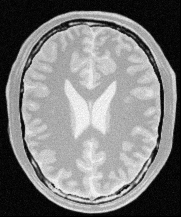
\includegraphics[width=0.25\textwidth]{itkExamplesIronPythonSpeedImage1Input.png}
	}
    \hspace{0.25mm}
	\subfigure[Speed Image Output]{
		
\includegraphics[width=0.25\textwidth]{itkExamplesIronPythonSpeedImage1Output.png}
	}
    \caption{Output from \code{Examples/IronPython/IronPythonSpeedImage1.py}.}
	\label{fig:ExamplesIronPythonSpeedImage1a}
\end{figure}
\fi


%----------------------------------------------------------------------%
% Section
%----------------------------------------------------------------------%
\section{Frequently Asked Questions (FAQ)}
\setcounter{secnumdepth}{1}

\subsection{Why do I need to install \code{vcredist\_x86}?}
ManagedITK is a set of C++/CLI wrapper classes around the native ITK code:
it is not 100\% managed code.
As a result of using the C++/CLI Interop mechanism for mixing native and
managed code, all ManagedITK objects depend on the \code{x86\_Microsoft.VC80.CRT}
side-by-side assemblies.
The \code{vcredist\_x86} executable packages these dependencies and
installs them to the \code{C:/Windows/WinSxS} directory.
The pre-compiled assemblies were compiled with Visual Studio 8.0 SP1,
and therefore the SP1 version of \code{vcredist\_x86} \textbf{must} be used
(which is included with the pre-compiled 
assemblies)\footnote{Microsoft has not yet release a version of
\code{vcredist\_x86} SP1. However the RTM version can be downloaded
\href{http://www.microsoft.com/downloads/details.aspx?displaylang=en&FamilyID=32BC1BEE-A3F9-4C13-9C99-220B62A191EE}{here}.}.

\subsection{Does ManagedITK work with Mono?}
As far we know, ManagedITK will not work with Mono
(and hence on Linux platforms supporting by Mono).
ManagedITK is not 100\% managed code, it depends on the
\code{x86\_Microsoft.VC80.CRT} side-by-side assemblies.
This dependency (as far as we know\ldots) binds it to the Windows platform.
There has been some talk of migrating WrapITK (a totally separate project)
to a pure SWIG implementation which could allow for the generation of 100\% 
pure C\# wrappers (which would probably be compatible with Mono).

\subsection{Are all ManagedITK objects managed wrappers around native objects?}
No, not all ManagedITK objects are managed wrappers around native ITK objects.
To simplify the use of common objects most of the objects in the \code{ManagedITK.Common}
assembly are 100\% managed
(except for the explicit \code{itkImage} types eg. \code{itkImage\_UC2}).
Unfortunately, this design decision has resulted in performance issues with the
\code{ManagedITK.Image.Iterators} assembly, meaning the line between the managed and native
worlds may have to be moved in the near future.

\subsection{How do I use the ManagedITK assemblies?}
Section~\ref{sec:UsingPreCompiledAssemblies} explains how to use the
pre-compiled ManagedITK assemblies.
Basically you create a project, right-click ``References'',
select ``Add Reference...'',
browse to the location containing the ManagedITK assemblies,
select the desired assemblies (ensuring to always select \code{ManagedITK.Common.dll}),
and click ``OK''.
The \code{Examples} folder contains numerous projects using
the ManagedITK assemblies in this manner. 

\subsection{How do I determine the \code{types} parameter for \code{New()} methods?}
All natively wrapped objects have two types of wrappers: explicit-type wrappers
(eg. \code{itkThresholdImageFilter\_IF2}) and runtime-type wrappers
(eg. \code{itkThresholdImageFilter}). 
The runtime-type wrappers require a valid sequence of type parameters passed
into the \code{New()} method.

You can determine which parameters to pass the \code{New()} method by inspecting
the explicit-type wrappers in the Object Browser.
To open the Object Browser in Visual Studio select \code{View$>$Object Browser}.
Expand the desired assembly and scroll to the explicit-type wrappers for the
filter or object.
In the above example the \code{itkThresholdImageFilter} has a number of
explicit types: 
\code{itkThresholdImageFilter\_IF2},
\code{itkThresholdImageFilter\_IF3},
\code{itkThresholdImageFilter\_UC2},
\code{itkThresholdImageFilter\_UC3},
etc.
The suffix (ie. ``IF2'') indicates it expects a single image type to be
passed to the \code{New()} method.

Some more complex examples include 
\code{itkAddImageFilter} which expects three images
(indicated by the ``IF2IF2IF2'' suffix)
or
\code{itkLinearInterpolateImageFunction} which expects one image and
a pixel type (indicated by the ``IF2D'' suffix).
See \code{Examples/Interpolators/itk.Examples.Interpolators.Linear1.cs}
for an example.

\subsection{How do I monitor ITK events?}
Common native ITK events
(ie. Started, Ended, Aborted, Modified, Iteration, and Progress)
have been exposed as managed events.
To monitor the managed event, simply use a \code{delegate} to attach an observer.
See Section~\ref{sec:Examples:Sigmoid1} for an in-depth example.

\subsection{Why is my \code{ImageIterator} so slow?}
It is a known issue that \code{ImageIterator} objects in ManagedITK are slow.
This results from the managed-to-native transition which occurs
when incrementing the iterator.
The problem may be alleviated in the future by simplifying or removing
the \code{itkPixel} class.
In the meantime --- if speed is an issue for your application ---
you might consider creating a native custom filter and wrapping it
using an external project.

\subsection{How do I use ManagedITK and OpenGL?}
ManagedITK can be easily integrated with OpenGL using Tao
(Tao a set of .NET wrappers around OpenGL functions created as part of the Mono project).
Go to \href{http://taoframework.com}{http://taoframework.com} to download the latest
assemblies.

\subsection{How do I use ManagedITK and VTK?}
ManagedITK can be integrated with VTK using a VTK .NET wrapper,
of which at least two currently exist:
\href{http://vtkdotnet.sourceforge.net}{http://vtkdotnet.sourceforge.net}
or
\href{http://herakles.zcu.cz/research/vtk.net}{http://herakles.zcu.cz/research/vtk.net}.
An external project is supplied within the \code{Examples/ExternalProjects/VTK}
folder which provides wrappers for \code{ImageToVTKImageFilter} and
\code{VTKImageToImageFilter}.
View the \code{Readme.txt} file in the project directory for build instructions.

\subsection{How do I show an image using \code{System.Drawing.Bitmap}?}
See Section~\ref{sec:Examples:Bitmap1} which walks through
\code{Examples/Images/itk.Examples.Images.FormBitmap1.cs}.

\subsection{How do I wrap an external project?}
There will probably come a time when you want to wrap one of your
newly created customised filters.
Rather than integrate this into the ManagedITK source structure,
an external project mechanism (similar to WrapITK) has been provided.

The \code{Examples/ExternalProjects/Skeletonize} folder contains an example
of using such an external project.
In this example we wrap a distance-ordered homotopic thinning filter 
taken from the Insight Journal \cite{Lamy2006a}.

The first step is to create a \code{CMakeLists.txt} file specifying
that we are using ManagedITK to wrap an external project.
An important aspect to note is the setting of \emph{both} the
group and subgroup names (``\code{Image}'' and ``\code{Topology}''
in this example).
\lstset@make
\begin{center}
	\lstinputlisting
	{../Examples/ExternalProjects/Skeletonize/CMakeLists.txt}
\end{center}

The next step is to create a CMake file to wrap each class.
In our example we created two such files:
\code{managed\_itkChamferDistanceTransformImageFilter.cmake} and
\code{managed\_itkSkeletonizeImageFilter.cmake}.
Each CMake wrapper file must specify the class to wrap,
the template parameters,
and the managed methods/properties to emit.
Look through the \code{Source/Modules} 
folders for other examples of such files.
\lstset@make
\begin{center}
	\lstinputlisting
	{../Examples/ExternalProjects/Skeletonize/managed_itkSkeletonizeImageFilter.cmake}
\end{center}

Next, open CMake and point it to the external project folder,
and configure. Run the \code{FinishCMake.bat} file created in the
external project folder and then open the generated solution file.
Choose the build type (eg. Debug, Release, etc.) and build the
project.

%----------------------------------------------------------------------%
% Conclusion
%----------------------------------------------------------------------%
\section{Conclusion}
This article presented ManagedITK: a set of .NET wrappers for the Insight
Toolkit (ITK).
These wrappers have a number of nice features including:
support for all CLR languages (including C\#, VB.NET, and IronPython),
the ability to rapidly prototype graphical user interfaces using Windows Forms,
and simplified event handling.
Various examples were discussed.
Future development should focus on the issue of reducing the managed-to-native
transition overhead (particularly for \code{ImageIterator} objects),
increasing the coverage 
(especially to include support for complex IO, meshes, point sets,
and deformable registration),
and adding automated regression tests.
For suggestions, additions or bugs, feel free to contact 
us\footnote{Corresponding author: Dan Mueller: %
\href{mailto:dan.muel@gmail.com}{dan.muel@gmail.com} or
\href{mailto:dan.mueller@philips.com}{dan.mueller@philips.com}.}.

%======================================================================%
%                    B i b l i o g r a p h y                           % 
%======================================================================%
\newpage
\bibliographystyle{plain}
\bibliography{article}

\end{document}